
{\actuality}

Неотъемлемой особенностью токамака как системы удержания плазмы является то, что ограниченная плазма должна пропускать значительный ток, а соответствующая магнитная энергия больше, чем кинетическая энергия частиц, несущих ток. Объемные электроны являются носителями тока в термоядерной плазме при номинальных условиях, однако скорость электронного потока намного меньше, чем тепловые скорости электронов. Однако при некоторых условиях происходит так что небольшая популяция электронов с высокой надтепловой температурой становится значительным или даже доминирующим носителем тока. Основная причина такого явления заключается в том, что сила трения для быстрых электронов уменьшается с увеличением скорости. Электроны могут при этом претерпевать неограниченное ускорение электрическим полем; находящиеся в таком режиме электроны называют убегающими. Убегающие электроны (УЭ) долгое время были предметом пристального внимания в исследованиях плазмы как по академическим, так и по практическим причинам. Они могут вызывать пробой газа в сильных электрических полях, в том числе при атмосферных молниях, они могут присутствовать в событиях магнитного перезамыкания и могут генерироваться намеренно для создания пучков электронов высокой энергии. Многие аспекты физики электронного пучка и взаимодействия пучка с плазмой естественным образом относятся к поведению УЭ. Одним из таких аспектов является возбуждение волн быстрыми электронами либо в форме спонтанного нетеплового излучения, либо в виде вынужденного излучения, ведущего к электронным неустойчивостям \autocite{Breizman2019}.

Столкновительные процессы для убегающих электронов играют намного меньшую роль, чем для основной массы электронов плазмы, поэтому их распределение по энергии существенно отличается от максвелловского. Ещё ранние теоретические исследования установили два механизма возникновения убегающих электронов: уход электронов из максвелловского хвоста в зону убегания и вторичные столкновения, которые увеличивают популяцию убегающих электронов в геометрической прогрессии. Убегающие электроны повсеместно присутствуют в плазме во время электрического пробоя газа в самом начале разряда, но их ток обычно остается относительно небольшим к тому времени, когда плазма нагревается и становится хорошим проводником, после чего они постепенно тк или иначе исчезают. Завершение разряда в штатных режимах работы обычно не вызывает повторного рождения убегающих электронов, однако если время отключения должно быть очень коротким в аварийной ситуации, то убегающие электроны во время гашения разряда становятся уже достаточно многочисленны (\autocite{Breizman2019}). На токамаке JET ток УЭ в процессе срыва может достигать значений 1~МА и выше и составлять 70\% и выше от полного тока по плазме \autocite{Smith2006}. На более крупных токамаках, таких как ИТЭР, следует ожидать ещё больших значений величины тока УЭ; так, согласно данным численного моделирования, величина тока УЭ на токамаке ИТЭР в некоторых сценариях может превышать 10~МА \autocite{Smith2006}. При этом пучок убегающих электронов может повреждать конструктивные элементы термоядерных реакторов (\autocite{Bazylev2011}, рисунок \cref{fig:electrons-wall}).

\begin{figure}[ht]
  \centerfloat{ 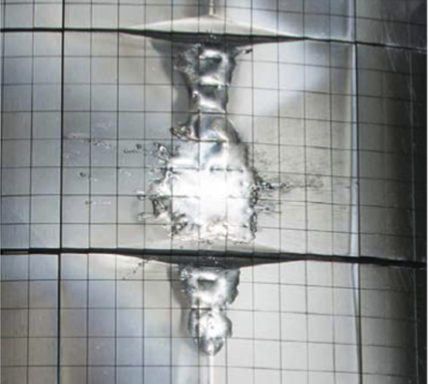
\includegraphics[width=0.80\linewidth]{electrons-wall} }
  \caption{ Повреждения внутренней стенки токамака JET пучком убегающих электронов (\autocite{Matthews2016}).}
  \label{fig:electrons-wall}
\end{figure}

В более крупных токамаках, таких как ИТЭР, токи и энергии пучка убегающих электронов будут ещё выше. Так, согласно требованиям к диагностике убегающих электронов, возможные значения энергии составляют до 100~МэВ, а значения тока - до 70\% от полного тока по плазме \autocite{Donne2007}. 

Эмиссия тормозного излучения --- один из наиболее широко используемых диагностических инструментов для диагностики убегающих электронов в токамаках \autocite{Breizman2019,Knoepfel1979}. Замедляясь в веществе, убегающие электроны генерируют тормозное излучение, энергия которого приходится на диапазон от дисятков кэВ до десятков МэВ и выше \autocite{Shevelev2014}. Тормозное излучение от УЭ может быть объемным тормозным излучением <<тонкой мишени>>, когда УЭ рассеивается ионами плазмы, или тормозным излучением <<толстой мишени>>, когда УЭ сталкиваются с материалами камеры токамака, обращенными к плазме. Объемная эмиссия доминирует, когда УЭ хорошо удерживаются, тогда как поверхностное тормозное излучение преобладает во время быстрого выхода УЭ на внутреннюю поверхность токамака в связи с МГД неустойчивостями, или если линия обзора спектрометра пересекает лимитер, а так же в некоторых других случаях \autocite{Breizman2019}. 

Тормозное излучение убегающих электронов может быть зарегистрированно с помощью сцинтилляционных детекторов, таких как NaI(Ti), BGO, LaBr3(Ce). От детекторов требуется регистрировать излучение в большом диапазоне энергий (от десятков-сотен кэВ и до дестятков МэВ), а так же с работать в том числе с высокой скоростью счёта (до $10^5$ -- $10^6$ c${}^-1$ и выше); дететоры должны работать в магнитных полях. На крупных токамаках, таких как ИТЭР, так же присутствуют и другие факторы: высокая температура и нейтронные поля в местах установки детекторов рентгеновского излучения. Зарегистрированный спектр рентгеновского излучения сложным образом зависит от функции распределения электронов, генерирующих излучение, от параметров конструктивных элементов, находящихся между источником излучения и детектором, а так же от аппаратной функции самого детектора. Таким образом, определение параметров пучка убегающих электронов и восстановление их функции распределения по энергии представляет собой непростую задау. 

Большие токамаки, такие как JET и ASDEX Upgrade, представляют собой несомненный интерес в плане изучения убегающих электронов. В отличие от малых токамаков, в больших установках есть возможность регистрировать тормозное рентгеновское излучение не от взаимодействия пучка электронов со стенкой (то есть от уже покинувших объём плазмы), а непосредственно из плазмы, что позволяет исследовать эволюцию пучка во времени. Кроме того, крупные установки являются хорошим испытательным стендом для отработки методик, которые могут быть применены на будущих крупных токамаках, таких как ИТЭР. 


% {\progress}
% Этот раздел должен быть отдельным структурным элементом по
% ГОСТ, но он, как правило, включается в описание актуальности
% темы. Нужен он отдельным структурынм элемементом или нет ---
% смотрите другие диссертации вашего совета, скорее всего не нужен.


{\aim} данной работы является развитие и практическое применение методов гамма-спектрометрии для исследования характеристик убегающих электронов в плазме токамаков.

Для~достижения поставленной цели необходимо было решить следующие {\tasks}:
\begin{enumerate}[beginpenalty=10000] % https://tex.stackexchange.com/a/476052/104425
  \item Развить методы обработки сигналов гамма-спектроскопии, полученных в ходе измерений спектров жесткого рентгеновского излучения в плазменных экспериментах, с целью уменьшения числа просчётов (мёртвого времени) и увеличения стабильности измеряемого сигнала. Реализовать разработанные методы в программном коде;
  \item Разработать методы восстановления функции распределения убегающих электронов по измеренному спектру рентгеновского излучения. Реализовать разработанные методы в программном коде;
  \item Разработать гамма-спектрометр на основе детектора LaBr3(Ce) для диагностики убегающих электронов на токамаке ASDEX Upgrade;
  \item Исследовать с помощью методов гамма-спетрометрии поведение убегающих электронов на токамаках JET и Asdex Upgrade.
\end{enumerate}

\textbf{Объект исследования:} убегающие электроны в плазме токамаков с энергией от 0.2~МэВ до 30~МэВ.

{\novelty}
\begin{enumerate}[beginpenalty=10000] % https://tex.stackexchange.com/a/476052/104425
  \item Развиты и реализованы в программном коде методы цифровой обработки сигналов, позволяющие осуществлять измерения спектра гамма и рентгеновского излучения с сцинтиляционных детекторов на основе кристаллов LaBr${}_3$(Ce) при скорости счётра 10${}^7$ и выше;
  \item Развиты и реализованы в программном коде методы восстановления функции распределения убегающих электронов по энергии на основе спектров излучения, зарегистрированных с помощью сцинтиляционных детекторов;
  \item Про детектор на ASDEX;
  \item Про выводы на токамаках Jet, Asdex.
\end{enumerate}

{\influence}\begin{enumerate}[beginpenalty=10000]
  \item Создан программный код DeGaSum, в котором были реализованы разработанные методы обратоки сигналов с детекторов, а так же методы восстановления функции распределения убегающих электронов. Данный код  применяется при обработке экспериментальных данных на токамаках JET, Asdex Upgrade, а так же Глобус-М2, Туман-3М, ФТ-2;
  \item Разработан гамма спектрометр на основе детектора LaBr3(Ce), который применялся для диагностики убегающих электронов на токамаке ASDEX Upgrade;
  \item Разработанные методики обработки гамма и рентгеновского излучения могут быть применены на токамаках нового поколения, включая ИТЭР и ТРТ.
\end{enumerate}

{\methods} 

{\defpositions}
\begin{enumerate}[beginpenalty=10000] % https://tex.stackexchange.com/a/476052/104425
  \item Методы цифровой обработки и амплитудного анализа сигнала сцинтилляционного гамма-детектора с использованием процедуры разделения наложенных импульсов реализованы в программном коде;
  \item Разработаны и реализованы в программном коде алгоритмы восстановления энергетического распределения быстрых (убегающих) электронов по измеренному жесткому рентгеновскому излучению из плазмы токамаков;
  \item Разработан гамма-спектрометр на основе детектора LaBr3(Ce) для диагностики убегающих электронов на токамаке ASDEX Upgrade;
  \item Получены результаты исследования эволюции максимальной энергии убегающих электронов по спектрам жесткого рентгеновского излучения в разрядах с массивной газовой инжекцией на токамаках ASDEX Upgrade и JET;
  \item Получены результаты исследования эволюции максимальной энергии и тока убегающих электронов по спектрам жесткого рентгеновского излучения на стадии подъема тока на токамаке JET.
\end{enumerate}

%В папке Documents можно ознакомиться с решением совета из Томского~ГУ
%(в~файле \verb+Def_positions.pdf+), где обоснованно даются рекомендации
%по~формулировкам защищаемых положений.

% {\reliability} полученных результатов обеспечивается \ldots \ Результаты находятся в соответствии с результатами, полученными другими авторами.


{\probation}
Основные результаты работы докладывались~на:
перечисление основных конференций, симпозиумов и~т.\:п.

{\contribution} Автор принимал активное участие \ldots

\ifnumequal{\value{bibliosel}}{0}
{%%% Встроенная реализация с загрузкой файла через движок bibtex8. (При желании, внутри можно использовать обычные ссылки, наподобие `\cite{vakbib1,vakbib2}`).
    {\publications} Основные результаты по теме диссертации изложены
    в~XX~печатных изданиях,
    X из которых изданы в журналах, рекомендованных ВАК,
    X "--- в тезисах докладов.
}%
{%%% Реализация пакетом biblatex через движок biber
    \begin{refsection}[bl-author, bl-registered]
        % Это refsection=1.
        % Процитированные здесь работы:
        %  * подсчитываются, для автоматического составления фразы "Основные результаты ..."
        %  * попадают в авторскую библиографию, при usefootcite==0 и стиле `\insertbiblioauthor` или `\insertbiblioauthorgrouped`
        %  * нумеруются там в зависимости от порядка команд `\printbibliography` в этом разделе.
        %  * при использовании `\insertbiblioauthorgrouped`, порядок команд `\printbibliography` в нём должен быть тем же (см. biblio/biblatex.tex)
        %
        % Невидимый библиографический список для подсчёта количества публикаций:
        \printbibliography[heading=nobibheading, section=1, env=countauthorvak,          keyword=biblioauthorvak]%
        \printbibliography[heading=nobibheading, section=1, env=countauthorwos,          keyword=biblioauthorwos]%
        \printbibliography[heading=nobibheading, section=1, env=countauthorscopus,       keyword=biblioauthorscopus]%
        \printbibliography[heading=nobibheading, section=1, env=countauthorconf,         keyword=biblioauthorconf]%
        \printbibliography[heading=nobibheading, section=1, env=countauthorother,        keyword=biblioauthorother]%
        \printbibliography[heading=nobibheading, section=1, env=countregistered,         keyword=biblioregistered]%
        \printbibliography[heading=nobibheading, section=1, env=countauthorpatent,       keyword=biblioauthorpatent]%
        \printbibliography[heading=nobibheading, section=1, env=countauthorprogram,      keyword=biblioauthorprogram]%
        \printbibliography[heading=nobibheading, section=1, env=countauthor,             keyword=biblioauthor]%
        \printbibliography[heading=nobibheading, section=1, env=countauthorvakscopuswos, filter=vakscopuswos]%
        \printbibliography[heading=nobibheading, section=1, env=countauthorscopuswos,    filter=scopuswos]%
        %
        \nocite{*}
        %\nocite{Reux2022}
        %\nocite{Panontin2021}

        %
        {\publications} Основные результаты по теме диссертации изложены в~\arabic{citeauthor}~печатных изданиях,
        \arabic{citeauthorvak} из которых изданы в журналах, рекомендованных ВАК\sloppy%
        \ifnum \value{citeauthorscopuswos}>0%
            , \arabic{citeauthorscopuswos} "--- в~периодических научных журналах, индексируемых Web of~Science и Scopus\sloppy%
        \fi%
        \ifnum \value{citeauthorconf}>0%
            , \arabic{citeauthorconf} "--- в~тезисах докладов.
        \else%
            .
        \fi%
        \ifnum \value{citeregistered}=1%
            \ifnum \value{citeauthorpatent}=1%
                Зарегистрирован \arabic{citeauthorpatent} патент.
            \fi%
            \ifnum \value{citeauthorprogram}=1%
                Зарегистрирована \arabic{citeauthorprogram} программа для ЭВМ.
            \fi%
        \fi%
        \ifnum \value{citeregistered}>1%
            Зарегистрированы\ %
            \ifnum \value{citeauthorpatent}>0%
            \formbytotal{citeauthorpatent}{патент}{}{а}{}\sloppy%
            \ifnum \value{citeauthorprogram}=0 . \else \ и~\fi%
            \fi%
            \ifnum \value{citeauthorprogram}>0%
            \formbytotal{citeauthorprogram}{программ}{а}{ы}{} для ЭВМ.
            \fi%
        \fi%
        % К публикациям, в которых излагаются основные научные результаты диссертации на соискание учёной
        % степени, в рецензируемых изданиях приравниваются патенты на изобретения, патенты (свидетельства) на
        % полезную модель, патенты на промышленный образец, патенты на селекционные достижения, свидетельства
        % на программу для электронных вычислительных машин, базу данных, топологию интегральных микросхем,
        % зарегистрированные в установленном порядке.(в ред. Постановления Правительства РФ от 21.04.2016 N 335)
    \end{refsection}%
    \begin{refsection}[bl-author, bl-registered]
        % Это refsection=2.
        % Процитированные здесь работы:
        %  * попадают в авторскую библиографию, при usefootcite==0 и стиле `\insertbiblioauthorimportant`.
        %  * ни на что не влияют в противном случае
        %\nocite{*}
        %\insertbiblioauthor
        %\nocite{Reux2022}
        %\nocite{Panontin2021}
        %\nocite{vakbib2}%vak
        %\nocite{patbib1}%patent
        %\nocite{progbib1}%program
        %\nocite{bib1}%other
        %\nocite{confbib1}%conf

    \end{refsection}%
        %
        % Всё, что вне этих двух refsection, это refsection=0,
        %  * для диссертации - это нормальные ссылки, попадающие в обычную библиографию
        %  * для автореферата:
        %     * при usefootcite==0, ссылка корректно сработает только для источника из `external.bib`. Для своих работ --- напечатает "[0]" (и даже Warning не вылезет).
        %     * при usefootcite==1, ссылка сработает нормально. В авторской библиографии будут только процитированные в refsection=0 работы.
     %\nocite{*}
     %\nocite{Reux2022}
     %\nocite{Panontin2021}
}



\ifdefmacro{\microtypesetup}{\microtypesetup{protrusion=false}}{} % не рекомендуется применять пакет микротипографики к автоматически генерируемому списку литературы
\urlstyle{rm}                               % ссылки URL обычным шрифтом

          %  \begin{refcontext}[labelprefix=A]
              % -- отключаем!
              %      \insertbiblioauthor      % Вывод всех работ автора
         %   \end{refcontext}
        %\printbibliography[heading=nobibheading, section=0, env=countexternal, keyword=biblioexternal, resetnumbers=true]%
%    }
%}
\ifdefmacro{\microtypesetup}{\microtypesetup{protrusion=true}}{}
\urlstyle{tt}                               % возвращаем установки шрифта ссылок URL



